In a quantum computer information is stored in so-called \emph{qubits} (quantum bits), an analogy to classical bits. A qubit is a microscopic two-state quantum mechanical system, for example an electron with spin up or spin down or a photon with two perpendicular polarization states. These two states represent the computational basis \( \{\ket{0},\ket{1}\} \). So instead of either representing 0 or 1 like a classical bit, a qubit can be in both states simultaneously (a superposition of two states), for example \( \ket{\psi} = \alpha \ket{0} + \beta \ket{1} \). The wave functions are normalized: \( |\alpha|^2+|\beta|^2=1 \)

Multiple qubits form a \emph{Quantum Register}. Quantum registers can store several numbers at the same time, i.e. the system can be in all classical states at once. A quantum register consisting of \emph{n} qubits thus has \(2^n\) possible states. A quantum register of size four could be in state \( \ket{0110} \) but also in all other \( 2^4 = 16 \) states \( \{\ket{0000},\ket{0001}...\ket{1110},\ket{1111}\} \) at the same time.

The most general state for a \emph{n} qubit quantum register is thus

\begin{equation}
 \sum_{\mathbf{x}\in\{0,1\}^n} \alpha_x\ket{\mathbf{x}}
\end{equation}

Manipulations on qubits are done by unitary operations, these can be performed by \emph{quantum logic gates}. All quantum gates are reversible, in contrast to classical computers. Several quantum logic gates form a quantum network.

The gates can be represented by \(2^n\) by \(2^n\) matrices (where \emph{n} is the size of the quantum register) which act on the computational basis.

The computational basis of a two-qubit quantum register would be \( \ket{00}, \ket{01}, \ket{10}, \ket{11} \} \). So a gate acting on a register in state \( \ket{00} \) would be equivalent to multiplying the matrix by the vector

\begin{equation}
 \ket{00} =\{\ket{0} \otimes \ket{0} = \begin{pmatrix} 1 \\ 0 \end{pmatrix} \otimes \begin{pmatrix} 1 \\ 0 \end{pmatrix} = \begin{pmatrix} 1 \\ 0\\0\\0 \end{pmatrix}
\end{equation}

There are many equivalent ways to write multiple-qubit states \( \ket{\mathbf{x}} \) where \( \mathbf{x} \in \{0,1 \}^n \). For example

\begin{equation}
 \ket{\mathbf{x}} = \ket{3} = \ket{011} = \ket{0} \otimes \ket{1} \otimes \ket{1}
\end{equation}

One of the fundamental gates is the Hadamard gate. It is a unitary gate acting on one qubit and can be represented by the two-by-two matrix 

\begin{equation}
 H = \frac{1}{\sqrt{2}}
  \begin{pmatrix} 1 & 1 \\ 1 & -1 \\ \end{pmatrix}
\end{equation}

acting on the computational basis \(\{\ket{0},\ket{1}\}\) of the qubit.

\begin{figure}[H]
	\centering
	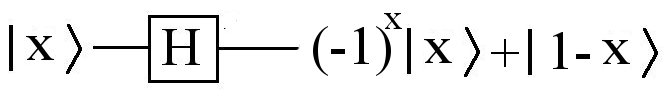
\includegraphics[width=50mm]{./images/hadamard}
	\caption{Graphical representation of the Hadamard gate}
\end{figure}

Another fundamental gate is the phase shift gate:

\begin{equation}
 \phi = \begin{pmatrix}	1 & 0 \\  0 & e^{ \imath \phi } \\ \end{pmatrix}
\end{equation}

A combination of two Hadamard and two phase shift gates can construct any unitary operation on a single qubit.

The phase shift gate is used in the Quantum Fourier Transform (QFT), a discrete Fourier transform applied to a quantum register. One of its uses is in Shor's algorithm, to put a quantum register in the superposition of all its states.

Thus for a quantum computer consisting of a single qubit the Hadamard and phase gate would be a universal set of operators, but a single qubit computer would not be of much use as the power of quantum computing lies in the entanglement of the qubits. This entanglement is done by multi-qubit gates consisting of control and target qubits. The simplest two-qubit gate is the “controlled NOT” gate (or C-NOT). The C-NOT gate is the reversible version of the classical (irreversible) XOR gate. It is made reversible by keeping the value of the control qubit. It is represented by the matrix

\begin{equation}
 C = \begin{pmatrix}
	1 & 0 & 0 & 0 \\
 	0 & 1 & 0 & 0 \\
	0 & 0 & 0 & 1 \\
	0 & 0 & 1 & 0
 	\end{pmatrix}
\end{equation}

\noindent acting on the computational basis \(\{\ket{00},\ket{01},\ket{10},\ket{11}\}\).

Another important two qubit gate is the controlled-V gate. Any unitary transformation acting on any number of qubits can be constructed by a network of only Hadamard and controlled-V gates. The controlled-V gate is represented by the matrix

\begin{equation}
 V = \begin{pmatrix}
	1 & 0 & 0 & 0 \\
 	0 & 1 & 0 & 0 \\
	0 & 0 & 1 & 0 \\
	0 & 0 & 0 & i
	 \end{pmatrix}
\end{equation}

The C-NOT gate and the C-V gate are both of the form controlled U. A control qubit is left unchanged, and a target qubit will be changed if the control qubit is in state \(\ket{1}\).

\begin{figure}[H]
	\centering
	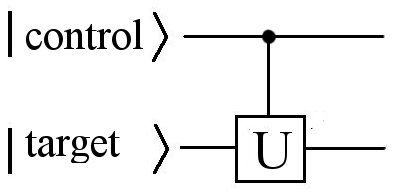
\includegraphics[width=35mm]{./images/cugate}
	\caption{Graphical representation of the controlled U gate}
\end{figure}

Another important gate for our simulation is the swap gate. It is a two-qubit gate that swaps two adjacent qubits and is represented by the matrix

\begin{equation}
 S = \begin{pmatrix}
	1 & 0 & 0 & 0 \\
 	0 & 0 & 1 & 0 \\
	0 & 1 & 0 & 0 \\
	0 & 0 & 0 & 1
 \end{pmatrix}
\end{equation}

The swap matrix can be used to swap qubits in a quantum register making control and target qubits adjacent. This helps when applying multiple-qubit gates like the C-NOT gate on non-adjacent qubits. The qubits can be swapped several times until they are adjacent. Then the C-NOT can be applied and afterwards they get swapped back to their original position. \cite{ekert2000, stolze2008}